\documentclass[12pt]{report}
\usepackage{graphicx}
\graphicspath{ {./images/} }

\title{{Progetto di Meccatronica}\\{Robotic sorter}}

\author{{Tosi Ubaldo}\\{Passerella Filippo}}

\begin{document}
\maketitle

\tableofcontents

\chapter{Introduzione}

Abbiamo realizzato il controllo di un manipolatore per smistamento di cubi colorati.

Il sistema riconosce il colore del cubo posto sull'apposita pedana e lo riposiziona nella zona appropriata. Poi torna alla posizione iniziale, in attesa del cubo seguente.

Abbiamo provato il sistema in più condizioni e non ci sono noti casi di malfunzionamento in ambiente adatto.

\section{Divisione delle funzioni}

Abbiamo deciso di dividere il programma finale in due parti, un modulo di percezione e un modulo di attuazione.

\begin{figure}
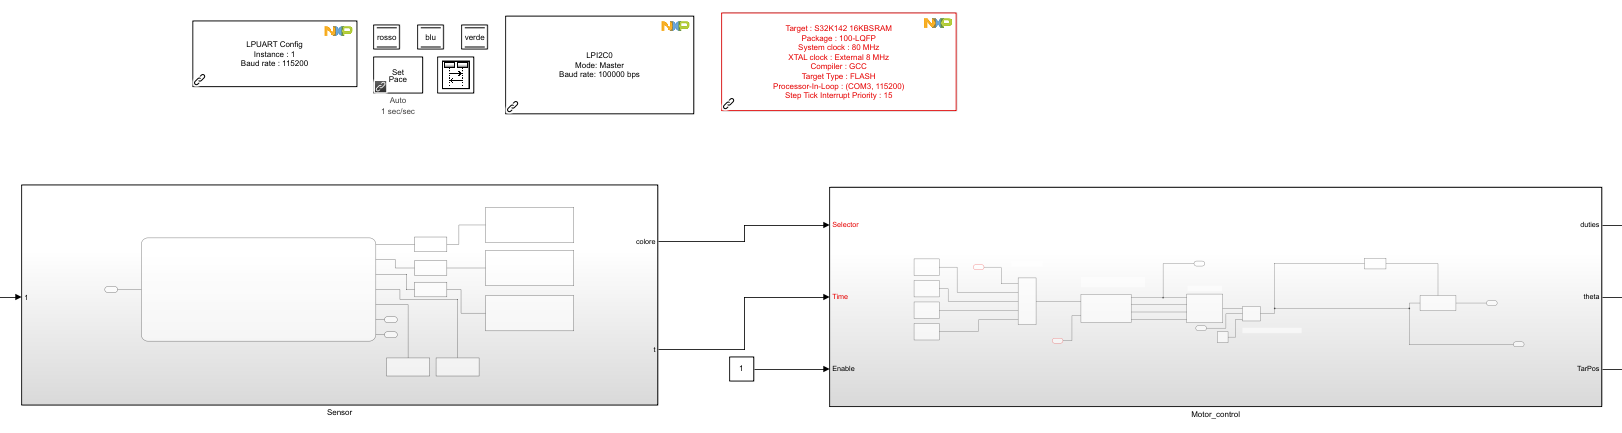
\includegraphics[width=\textwidth]{Modules}
\caption{Moduli}
\end{figure}

Il primo si occupa di interfacciarsi con il sensore di colore e temporizzare il secondo. Il secondo controlla il manipolatore e gestisce i percorsi.

Le funzioni dei due moduli erano sufficientemente indipendenti da poter essere sviluppati e verificati parallelamente.

Ottenuti dei prototipi funzionanti dei due moduli, abbiamo definito l'interfaccia che ha poi determinato la loro versione finale.

\section{Modalità d'uso}

Innanzitutto, occorre collegare l'hardware e accendere il dispositivo.

---------------Foto o tabella dei collegamenti

Si vedrà il braccio posizionarsi nella configurazione di attesa.

Posizionare un cubo colorato sulla pedana e premere \emph{sw2}.

Il manipolatore sposterà il cubo nella zona appropriata e tornerà nella configurazione di attesa.

\chapter{Percezione}


\chapter{Attuazione}

Il modulo di attuazione controlla l'uscita PWM per i servo-motori per guidare il braccio robotico lungo percorsi predefiniti.

Due input determinano il percorso da seguire e il punto corrente del percorso.

Altri input e output sono usati solo in fase di debug.

Il modulo è stato ideato per permettere un controllo semplice della velocità di esecuzione e flessibilità nella scelta del percorso.

\section{Principio di funzionamento}

\begin{figure}
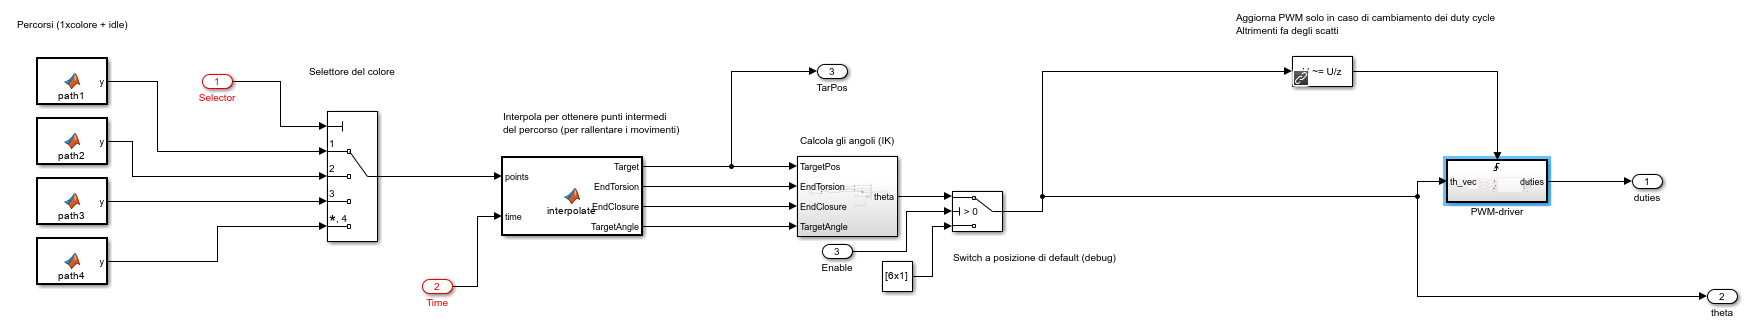
\includegraphics[width=\textwidth]{Complete_attuation}
\caption{Diagramma completo}
\end{figure}

I blocchi \textbf{Path1...Path4} restituiscono ognuno una matrice costante che rappresenta un percorso per il braccio robotico. Ogni riga rappresenta un punto chiave del percorso. A partire dai punti chiave vengono successivamete calcolati punti intermedi.

Ogni riga contiene 7 elementi:

\begin{itemize}
\item Distanza radiale in coordinate cilindriche dell'obiettivo dal centro della base del braccio robotico.
\item Angolo in cordinate cilindriche dell'obiettivo.
\item Distanza verticale in coordinate cilindriche dell'obiettivo dalla base del braccio robotico.
\item Angolo tra il vettore parallelo all'ultimo segmento del manipolatore (positivo verso la pinza) e la verticale (positiva verso l'alto).
\item Angolo del polso.
\item Angolo di chiusura della pinza.
\item Istante temporale del punto nel percorso.
\end{itemize}

\begin{figure}
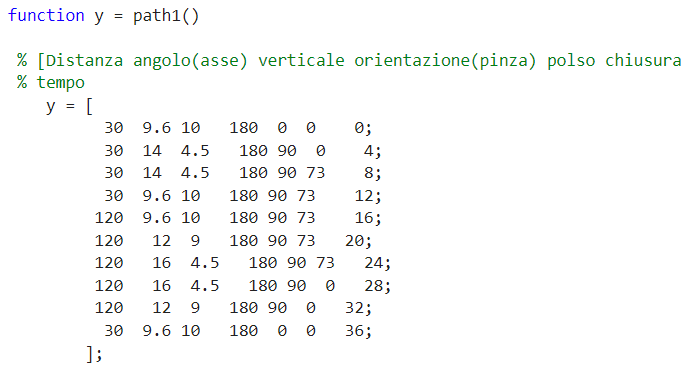
\includegraphics[width=\textwidth]{Path_structure}
\caption{Esempio di percorso}
\end{figure}

L'input \textbf{Selector} determina quale percorso verrà usato.

Il blocco \textbf{Interpolate} genera un punto intermedio interpolando linearmente due punti successivi nel percorso in base all'input \textbf{Time}.

Parte del blocco serve a garantire le corrette dimensioni della matrice in ingresso.

Vengono usati i punti estremi se \textbf{Time} eccede gli istanti temporali estremi.

Il blocco successivo calcola gli angoli dei servo-motori a partire dal punto interpolato.

Lo switch che segue permette di sostituire gli angoli calcolati con angoli predefiniti, per portare il manipolatore in una configurazione sicura durante il debug.

Il blocco \textbf{PWM-driver} imposta le uscite PWM a partire dagli angoli desiderati.

Questo blocco viene eseguito solo se gli angoli desiderati cambiano.

\section{Reimpostazione periodica del PWM}

Se il blocco \textbf{PWM-driver} venisse attivato liberamente (senza trigger al cambiamento) i servo-motori subirebbero uno scatto dovuto alla reimpostazione del PWM, che avviene anche quando i duty-cycle non variano.

Per questo è importante usare il blocco \textbf{Detect Change}. 

\section{Cinematica inversa}

Ci sono 6 motori in totale, denominati da M1 a M6.

M6 controlla la chiusura della pinza, M5 la rotazione del polso. I motori che determinano posizione e orientazione dell'end-effector sono 4.

M2, M3 e M4 possono spostare l'end-effector solo sul piano determinato da M1. Fissata la posizione dell'end-effector, è determinata la rotazione di M1 per avere l'allineamento. Fissata anche l'orientazione finale desiderata, anche la posizione di M4 è identificata. Data questa, M2 e M3 formano uno Scara con M4 come end-effector.

\section{Test}

Il sistema di attuazione è stato prima verificato in SIL e in PIL in più iterazioni.

Sono stati progressivamente aggiunti blocchi ad ogni iterazione che ha avuto successo, in questo ordine: PWM-driver, IK, Interpolate, Selector.

Le uscite di debug mostrano la posizione desiderata, gli angoli previsti e i duty cycle impostati.

Un input di debug permette di riportare il braccio in una posizione sicura ed è stato usato in PIL.

\begin{figure}
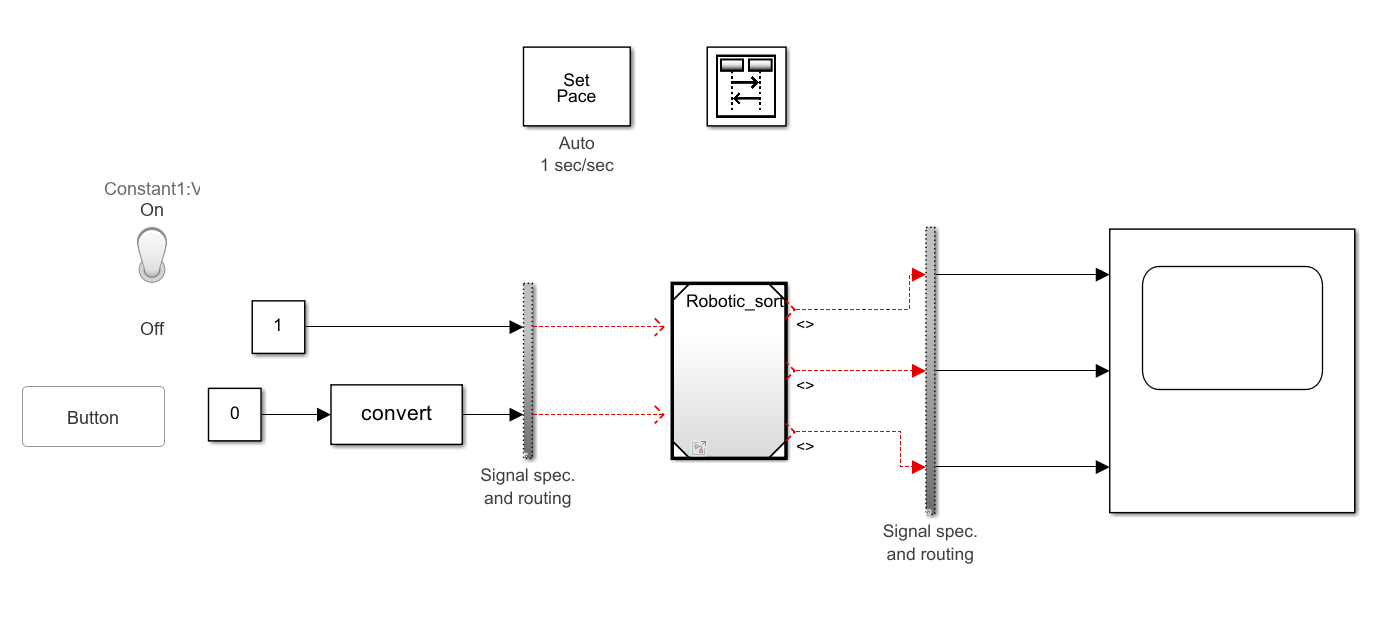
\includegraphics[width=\textwidth]{Harness}
\caption{Harness del modulo di attuazione (screenshot scattato a fine progetto, differisce parzialmente da quello usato.}
\end{figure}

\chapter{Verifica finale}

Sviluppati e verificati indipendentemente i due moduli, abbiamo cominciato la fase finale.

I due moduli sono stati combinati velocemente, grazie alla semplice interfaccia.

Ci siamo accorti di non poter fare simulazioni \emph{in the loop} perché incompatibili con la periferica I2C.

Abbiamo usato la UART per verificare che tutto proseguisse come previsto durante la verifica.

Non abbiamo riscontrato problemi oltre all'impossibilità di usare SIL/PIL o i timer (per mandare messaggi temporizzati tramite UART). Così abbiamo subito potuto definire e verificare i percorsi.

Avevamo preparato delle bozze dei percorsi usando un modello del braccio realizzato e animato su Blender3D. Modificando queste in base alle verifiche abbiamo ottenuto dei percorsi che ci soddisfacessero.

\begin{figure}
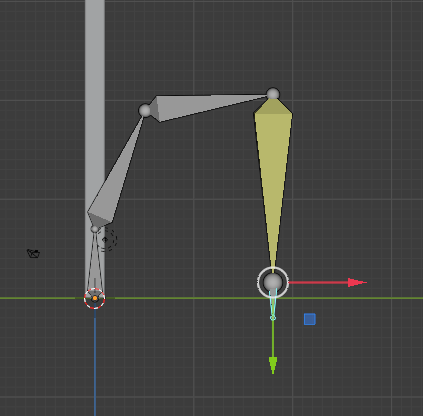
\includegraphics[width=\textwidth]{Blender3D}
\caption{Armatura del braccio su Blender3D}
\end{figure}

\chapter{Problemi durante lo sviluppo}

Durante i test PIL, due pezzi stampati 3D per la trasmissione della coppia da servo-motori a struttura si sono rotti. In particolare si sono spanati gli incastri per i servo-motori.

Il primo guasto è stato dovuto a un blocca di ritardo nell'harness: la condizione iniziale ha fatto piegare il braccio su se stesso all'avvio.

Il secondo guasto è stato dovuto alla base fissata male (svitando le viti si sono rovinati i fori) in seguito alle riparazioni del guasto precedente.

\chapter{Conclusione}

Realizzata la parte funzionale, abbiamo preparato una base pieghevole su cui abbiamo montato la pedana di riconoscimento e dei cartoncini colorati per indicare le zone di smistamento.

Riguardo la parte di attuazione, i due passaggi chiave sono stati la riduzione dell'algoritmo IK a quello di uno scara e l'uso estensivo di SIL e PIL.

Mentre per quanto riguarda la fase di percezione i passaggi chiave sono stati la scelta dei parametri del sensore con la scelta dei colori e finiture migliori dei cubi colorati, l'uso della UART per il debug e l'interpretazione di un voter.

------------------Bla bla bla

Noi possiamo ritenere con soddisfazione questo progetto un successo, dal punto di vista sia del risultato finale, sia della flessibilità e futura modificabilità della funzione, sia del processo in sé.
\end{document}